\documentclass[11pt,a4paper]{article}
\usepackage{amsmath}
\usepackage{amssymb}
\usepackage{graphicx}
\usepackage{subfigure}
\usepackage{float}
\usepackage{xeCJK}
\usepackage{geometry}
\geometry{left=2.0cm,right=2.0cm,top=2.0cm,bottom=2.0cm}

\usepackage{underscore}

\usepackage[T1]{fontenc}
\usepackage{xcolor}
\usepackage{lmodern}
\usepackage{listings}
\definecolor{mygreen}{rgb}{0,0.6,0}
\definecolor{mygray}{rgb}{0.5,0.5,0.5}
\definecolor{mymauve}{rgb}{0.58,0,0.82}

\lstset{
	basicstyle=\footnotesize,        % the size of the fonts that are used for the code
	breakatwhitespace=false,         % sets if automatic breaks should only happen at whitespace
	breaklines=false,                 % sets automatic line breaking
	captionpos=b,                    % sets the caption-position to bottom
	commentstyle=\color{mygreen},    % comment style
	extendedchars=true,              % lets you use non-ASCII characters; for 8-bits encodings only, does not work with UTF-8
	keepspaces=true,                 % keeps spaces in text, useful for keeping indentation of code (possibly needs columns=flexible)
	keywordstyle=\color{blue},       % keyword style
	language=[95]Fortran,                 % the language of the code
	numbers=left,                    % where to put the line-numbers; possible values are (none, left, right)
	numbersep=5pt,                   % how far the line-numbers are from the code
	numberstyle=\tiny\color{mygray}, % the style that is used for the line-numbers
	rulecolor=\color{black},         % if not set, the frame-color may be changed on line-breaks within not-black text (e.g. comments (green here))
	showspaces=false,                % show spaces everywhere adding particular underscores; it overrides 'showstringspaces'
	showstringspaces=false,          % underline spaces within strings only
	showtabs=false,                  % show tabs within strings adding particular underscores
	stepnumber=1,                    % the step between two line-numbers. If it's 1, each line will be numbered
	stringstyle=\color{mymauve},     % string literal style
	tabsize=4,                       % sets default tabsize to 2 spaces
	title=\lstname                   % show the filename of files
}


\title{MPI二维并行化}
\author{任广智}
\date{\today}

\begin{document}
	
\maketitle

首先考虑二维MPI通信域的建立,此处并不不涉及物理坐标,待通信域建立好之后,再将物理坐标对应进去就可以了。

MPI_DIMS_CREATE生成笛卡尔拓扑下的进程分布,需要注意的是,当dim_xy均为0时,系统自动划分进程分布。系统会尽量使每个维度上的进程数接近,而且dim_xy将以递减的顺序排序。当dim_xy的某个维度为正数时,这个维度不会被修改,系统仅修改其余为0的部分。
\begin{lstlisting}
call MPI_DIMS_CREATE(N_proces, 2, dim_xy(0:1), ierr)
\end{lstlisting}

以下的函数调用生成二维笛卡尔拓扑下的通信子域,并且生成相应的笛卡尔坐标便于使用。
\begin{lstlisting}
call MPI_CART_CREATE(MPI_comm_world, 2, dim_xy(0:1), period_xy(0:1), .false., &
		MPI_comm_cart_xy, ierr)
call MPI_CART_COORDS(MPI_comm_cart_xy, rank, 2, c_rank(0:1), ierr)
\end{lstlisting}

接下来我们考虑当考虑确切物理坐标以及网格数时候系统给出的二维MPI并行化方案。考虑实空间网格为$$(N_x,N_y,N_z)=(64,128,62)$$的情况,此时对应的经过P3DFFT变换之后的谱空间网格应为$$(N_x,K_y,K_z)=(64,128,32)$$
二维网格划分的关系则有
$$(\frac{N_x}{M_1},\frac{N_y}{M_2},N_z) \sim (N_x,\frac{N_y}{M1},\frac{N_z+2}{2M_2})=(N_x,\frac{K_y}{M1},\frac{K_z}{M_2})$$
令M1=dim_xy(1),M2=dim_xy(2)我们可以方便地得到每个进程中的网格数。也就是说我们将实空间中(Nx,Ny),谱空间中(Ky,Kz)分别对应到了dim_xy中。考虑8进程时候的情况,此时MPI给出的dim_xy=(4,2),相应的进程分布为:
\begin{figure}[H]
	\centering
	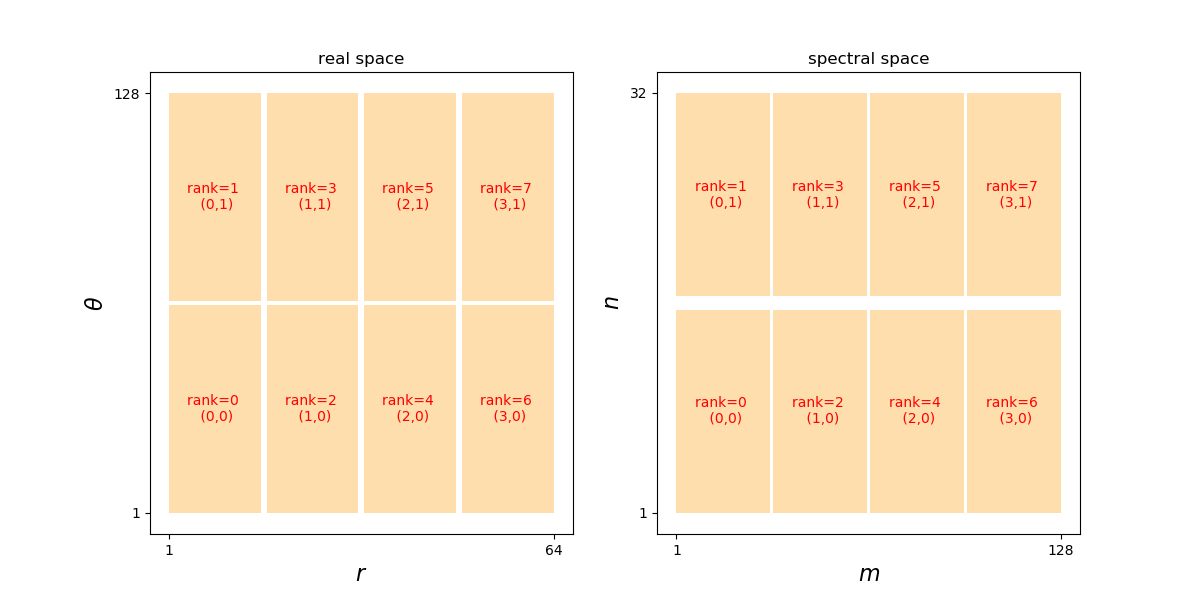
\includegraphics[width=0.8\textwidth]{./np8.png}
	\caption{}
\end{figure}
可以看出,网格的划分符合预期,实空间中径向为四进程,极向二进程,而谱空间中极向模数为四进程,环向模数为二进程。c_rank每个维度对应dim_xy的维度,也就是c_rank(0)对应径向,c_rank(1)对应极向。另外rank的排序为列主导,也就是说沿着c_rank(1)进行填充,这一点是很重要的。通过上述图片可以比较清楚地看到二维下的进程分布。相邻的进程互相交换数据,这个在程序中通过MPI_CART_SHIFT来完成。一维的通信子域的生成通过MPI_COMM_SPLIT来完成。

通过上述图像,我们知道内边界进程为c_rank(0)=0的进程,而外边界进程为c_rank(0)=dim_xy(0)-1的进程。对于需要交换关于圆心对称的内边界进程数据,我们将进程划分映射到极坐标下来观察。8进程下我们只需要交换进程0和进程1的边界数据即可。
\begin{figure}[H]
	\centering
	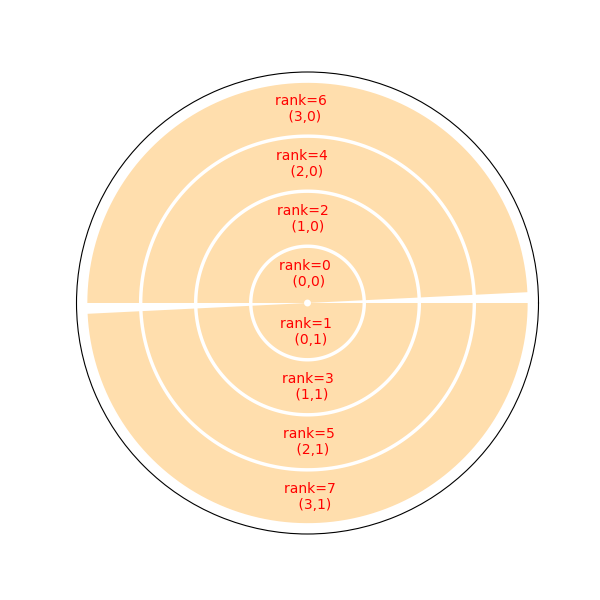
\includegraphics[width=0.4\textwidth]{./np8-p.png}
	\caption{}
\end{figure}
我们设置dim_xy=(2,16)下的情况。可以看到内边界需要交换的数据在c_rank(1)的数值上相差8,即dim_xy(1)/2。所以关于内边界的需要交换的进程我们定义为z_rank时,z_rank的定义应如下:
\begin{lstlisting}
    if(c_rank(0) == 0) then
		if(c_rank(1) <= dim_xy(1)/2-1) then
			z_rank = rank + dim_xy(1)/2
		else
			z_rank = rank - dim_xy(1)/2
		end if
	end if
\end{lstlisting}
\begin{figure}[H]
	\centering
	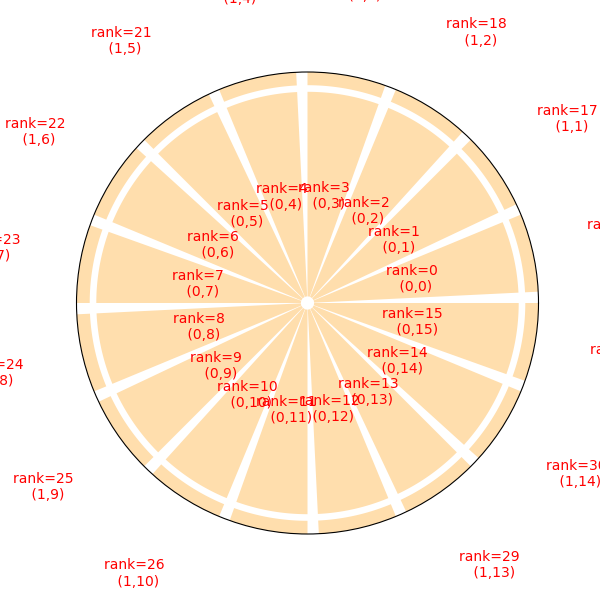
\includegraphics[width=0.4\textwidth]{./np32-p.png}
	\caption{}
\end{figure}


\end{document}






